%!TEX root = ../munich21.tex

\begin{frame}{Graph Laplacian}

	\note{The graph Laplacian has become a primary tool for the study of networks.
	\vk
	It is typically defined using the incidence matrix of a graph and the valence matrix of its nodes, but we can equivalently define it using the boundary matrix that gave us 1-homology. \press

	Here is the definition and an example illustrating it.
	\vk
	Naturally, we can set $W$ to be the identity if we are interested in unweighted networks. \press

	The spectrum of this matrix is an important feature of the network. \press

	Additionally, we can consider the eigenvectors of the graph Laplacian. This preferred basis is often used for signal analysis on graphs. \press

	Where \textit{signal} in this context means a real-valued function from the set of vertices of the graph. \press

	What if we are interested in signals defined not just on vertices but on sets of such vertices? But even earlier, are there any interesting signals defined on subsets of vertices?
	}

	A powerful tool to study weighted networks.

	\vskip 5pt
	\pause

	\begin{center}
		\includegraphics[scale=.5]{media/graph}
	\end{center}

	\vskip -5pt

	\begin{equation*}
	\resizebox{8.5cm}{!}{
		$\partial_1 =
		\begin{pmatrix*}[r]
		-1 & -1 &  0 \\
		 1 &  0 & -1 \\
		 0 &  1 &  1
		\end{pmatrix*}
		\qquad
		W =
		\begin{pmatrix*}[r]
		w_{01}& 0      & 0 \\
		0     & w_{01} & 0 \\
		0     &      0 & w_{12}
		\end{pmatrix*}
		\qquad
		\partial_1^{\mathrm T} =
		\begin{pmatrix*}[r]
		-1 &  1 & 0 \\
		-1 &  0 & 1 \\
		 0 & -1 & 1
		\end{pmatrix*}$}
	\end{equation*}

	\vskip 10pt
	\pause

	Two types of uses:
	\begin{itemize}
		\item[] \textcolor{pblue}{Structural (eigenvalues).} The spectrum as a feature of the graph.

		\pause

		\item[] \textcolor{pblue}{Functional (eigenvectors).} A Fourier basis for signals on the graph, \\

		\vskip 5pt
		\hspace*{5cm} \pause i.e., real numbers at every node.
	\end{itemize}

	\pause

	What if the signals are defined \\
	\textcolor{pblue}{\ \ \ not just on single nodes?}
\end{frame}

\begin{frame}{Information signals}

	\note{In the study of complex systems it is often said that the whole is more than the sum of its parts. \press

	But how can we quantify this?

	After Shannon's ground-breaking work on information theory. We have a well developed framework that allows us to compute the information content shared by different parts of the system, treated as subspaces of a join probability distribution. \press

	For us is not so important to go over these definitions. It suffices to know they exist, and, therefore, that natural signals properly defined over simplices of high dimensions exist.

	For example, to an edge we can assign the mutual information shared by it vertices, for triangles, the interaction information of its vertices, and to higher dimensional simplices, we can assign appropriate generalizations of these. \press

	\vk

	A practical problem though, is the large number of simplices we get as we increase the number of vertices.

	\vk

	Maybe we can \textit{compress} this signals into a lower dimensional space?

	}

	\textcolor{pblue}{Complex Systems:} The whole is greater than the sum of its parts.

	\begin{center}
		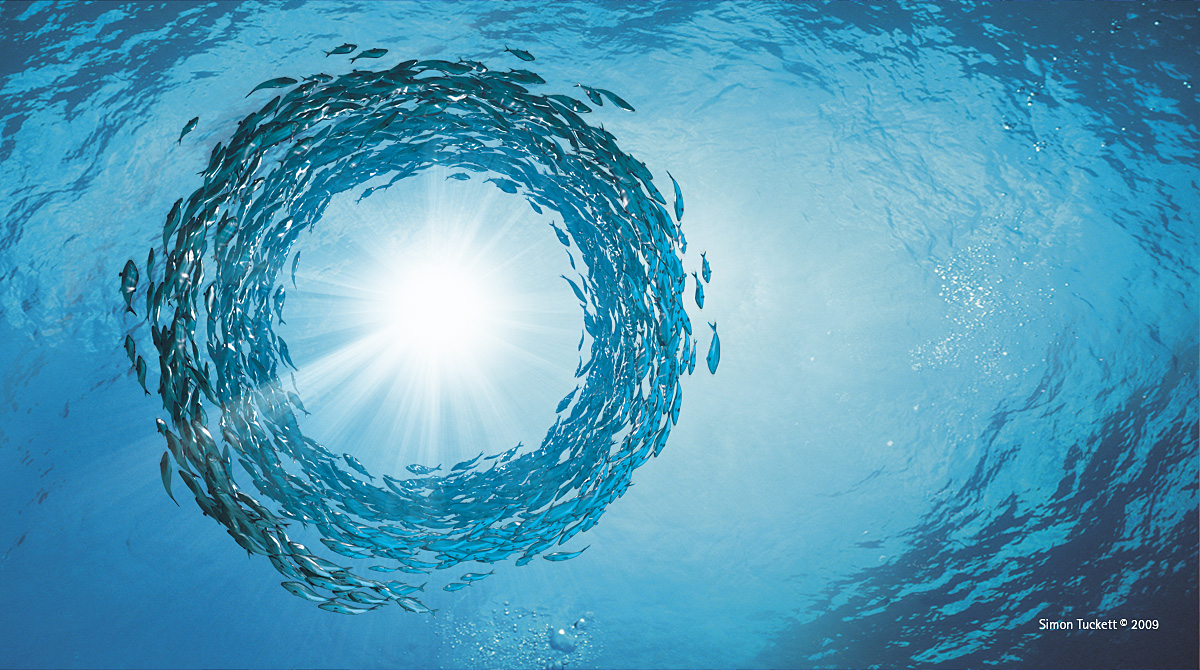
\includegraphics[scale=.12]{media/fishes}
	\end{center}

	\vskip 5pt
	\pause

	\textcolor{pblue}{But how to quantify this?}

	\vskip 5pt
	\pause

	Given collection of probability distributions $X_0, \dots, X_N$, can assign to

	\vskip 5pt

	\quad Pairs: their mutual information, \\
	\quad Triples: their interaction information, and\\
	\quad $(n+1)$-element sets: higher analogues of these.

	\vskip 5pt
	\pause

	\textcolor{pblue}{Problem:} The number of subsets grows exponentially with $N$.
\end{frame}

\begin{frame}{Hyperharmonic analysis}

	\note{Here is an analogy. Our cellphones are incapable of producing the fundamental frequency of most people's voices. But we still recognize them on the other side of the line, just hearing a lower fidelity version of their voices, that is, a lower dimensional representation of the signal. \press

	As another example, just a few harmonics are needed to distinguish a piano from a guitar playing the same note.

	Can we do something like that for information signals?

	Yes, indeed. \press

	Together with these researchers, we proposed a method that allows us to compress these signals substantially, reducing in this way some of the issues associated to the curse of dimensionality. \press

	As harmonic modes, we used the eigenvectors of a discrete analogue of the Laplace-de Rham operator of Riemannian geometry, which generalizes the graph Laplacian.

	And as a measure of compression, we use the cummulative explained variance, defined as follows. \press

	Consider a signal and a fix basis. Without loss of generality, order the coefficients of this signal, in that basis, so that their squares are non-increasing.
	The $k$-th explained variance is the proportion of the variance explained by the $k$-th coefficient, whereas the $k$-th cummulative explained variance is that explained by the first $k$ coefficients.
}

	\pause

	\vskip -5pt

	\textcolor{pblue}{Analogy:} We need only hear a few harmonics to distinguish a note played by a guitar or a piano.

	\vskip 5pt
	\pause

	\begin{result}
		Proposed a principled method to compress high-order information signals based on Fourier analysis and combinatorial topology.
	\end{result}

	Joint with F. Rosas (Imperial), S. Rodr\'iguez (UTFS) and R. Cofr\'e (PUCV).

	\vskip 15pt
	\pause

	\textcolor{pblue}{Discrete Laplacian:} $\displaystyle{L_n = \partial_{n+1} \partial_{n}^{\mathrm T} + \partial_{n-1}^{\mathrm T} \partial_{n}}$

	\vskip 15pt
	\pause

	\textcolor{pblue}{Compression:} $\alpha_1^2 \geq \alpha_2^2 \geq \cdots$ with $\{\alpha_i\}$ the coefficients in a basis.
	\begin{equation*}
	\text{EV}_{\alpha}(k) = \frac{ \alpha_k^2}{{\displaystyle \sum_{i} \alpha_i^2}}
	\qquad \text{ and } \qquad
	\text{CEV}_{\alpha}(k) = \sum_{1\leq i \leq k} \text{EV}_{\alpha}(i),
	\end{equation*}
\end{frame}

\begin{frame}{Proof of concept: Hadyn's symphonies}

	\note{\footnotesize
	As my last slide, let me show you some curves of the CEV obtained in a proof-of-concept example. \press

	We can think of a musical score as a multivariate time series, one time series for each instrument, and values between 0 and 12. This gives us a join probability distribution, based on the frequency of the notes.

	We considered the so called ``London symphonies" of Hadyn. \press

	And analysed two high-order generalization of Shannon's mutual information called O-information and S-information. These are proposed to respectively capture synergistic and redundant phenomena. Their interpretations will not play a role for us today, though.

	We computed them in dimension 2, 3, 4 and 5, corresponding to subsets of nodes of cardinalities between 3 and 6.

	And we then plotted the resulting CEV curves for the canonical basis and for the fourier basis. \press

	Here they are.

	\vk

	We can see that green and red reach high values very quickly. This tells us that with just a few coefficients in the fourier basis, we recover most of the signal. On the other hand, blue and orange require many more components to reach values close to 1, showing some of the advantges of the fourier basis over the canonical one, and based on a figure I am not showwing, also over randomly generated bases.

	\vk\vk
	--------------------


	Although, topology has been with mathematicians for over a century. In the past few years, we have seen an explosion of application of topology in the natural and computer sciences. And, thanks to the broader dissemination of \textit{its} ideas and the development of effective tools for its use, the insights that topology is providing researcher across diciplines are also... deepening.

	\vk

	With that said, I thank you very much for your time and attention.

}
	\vskip -5pt
	\pause

	Music as a probability distribution.

	\vskip 5pt
	\pause

	We analyzed two high-order information signals: O-info and S-info.

	\vskip 7pt
	\pause

	\hspace*{-15pt}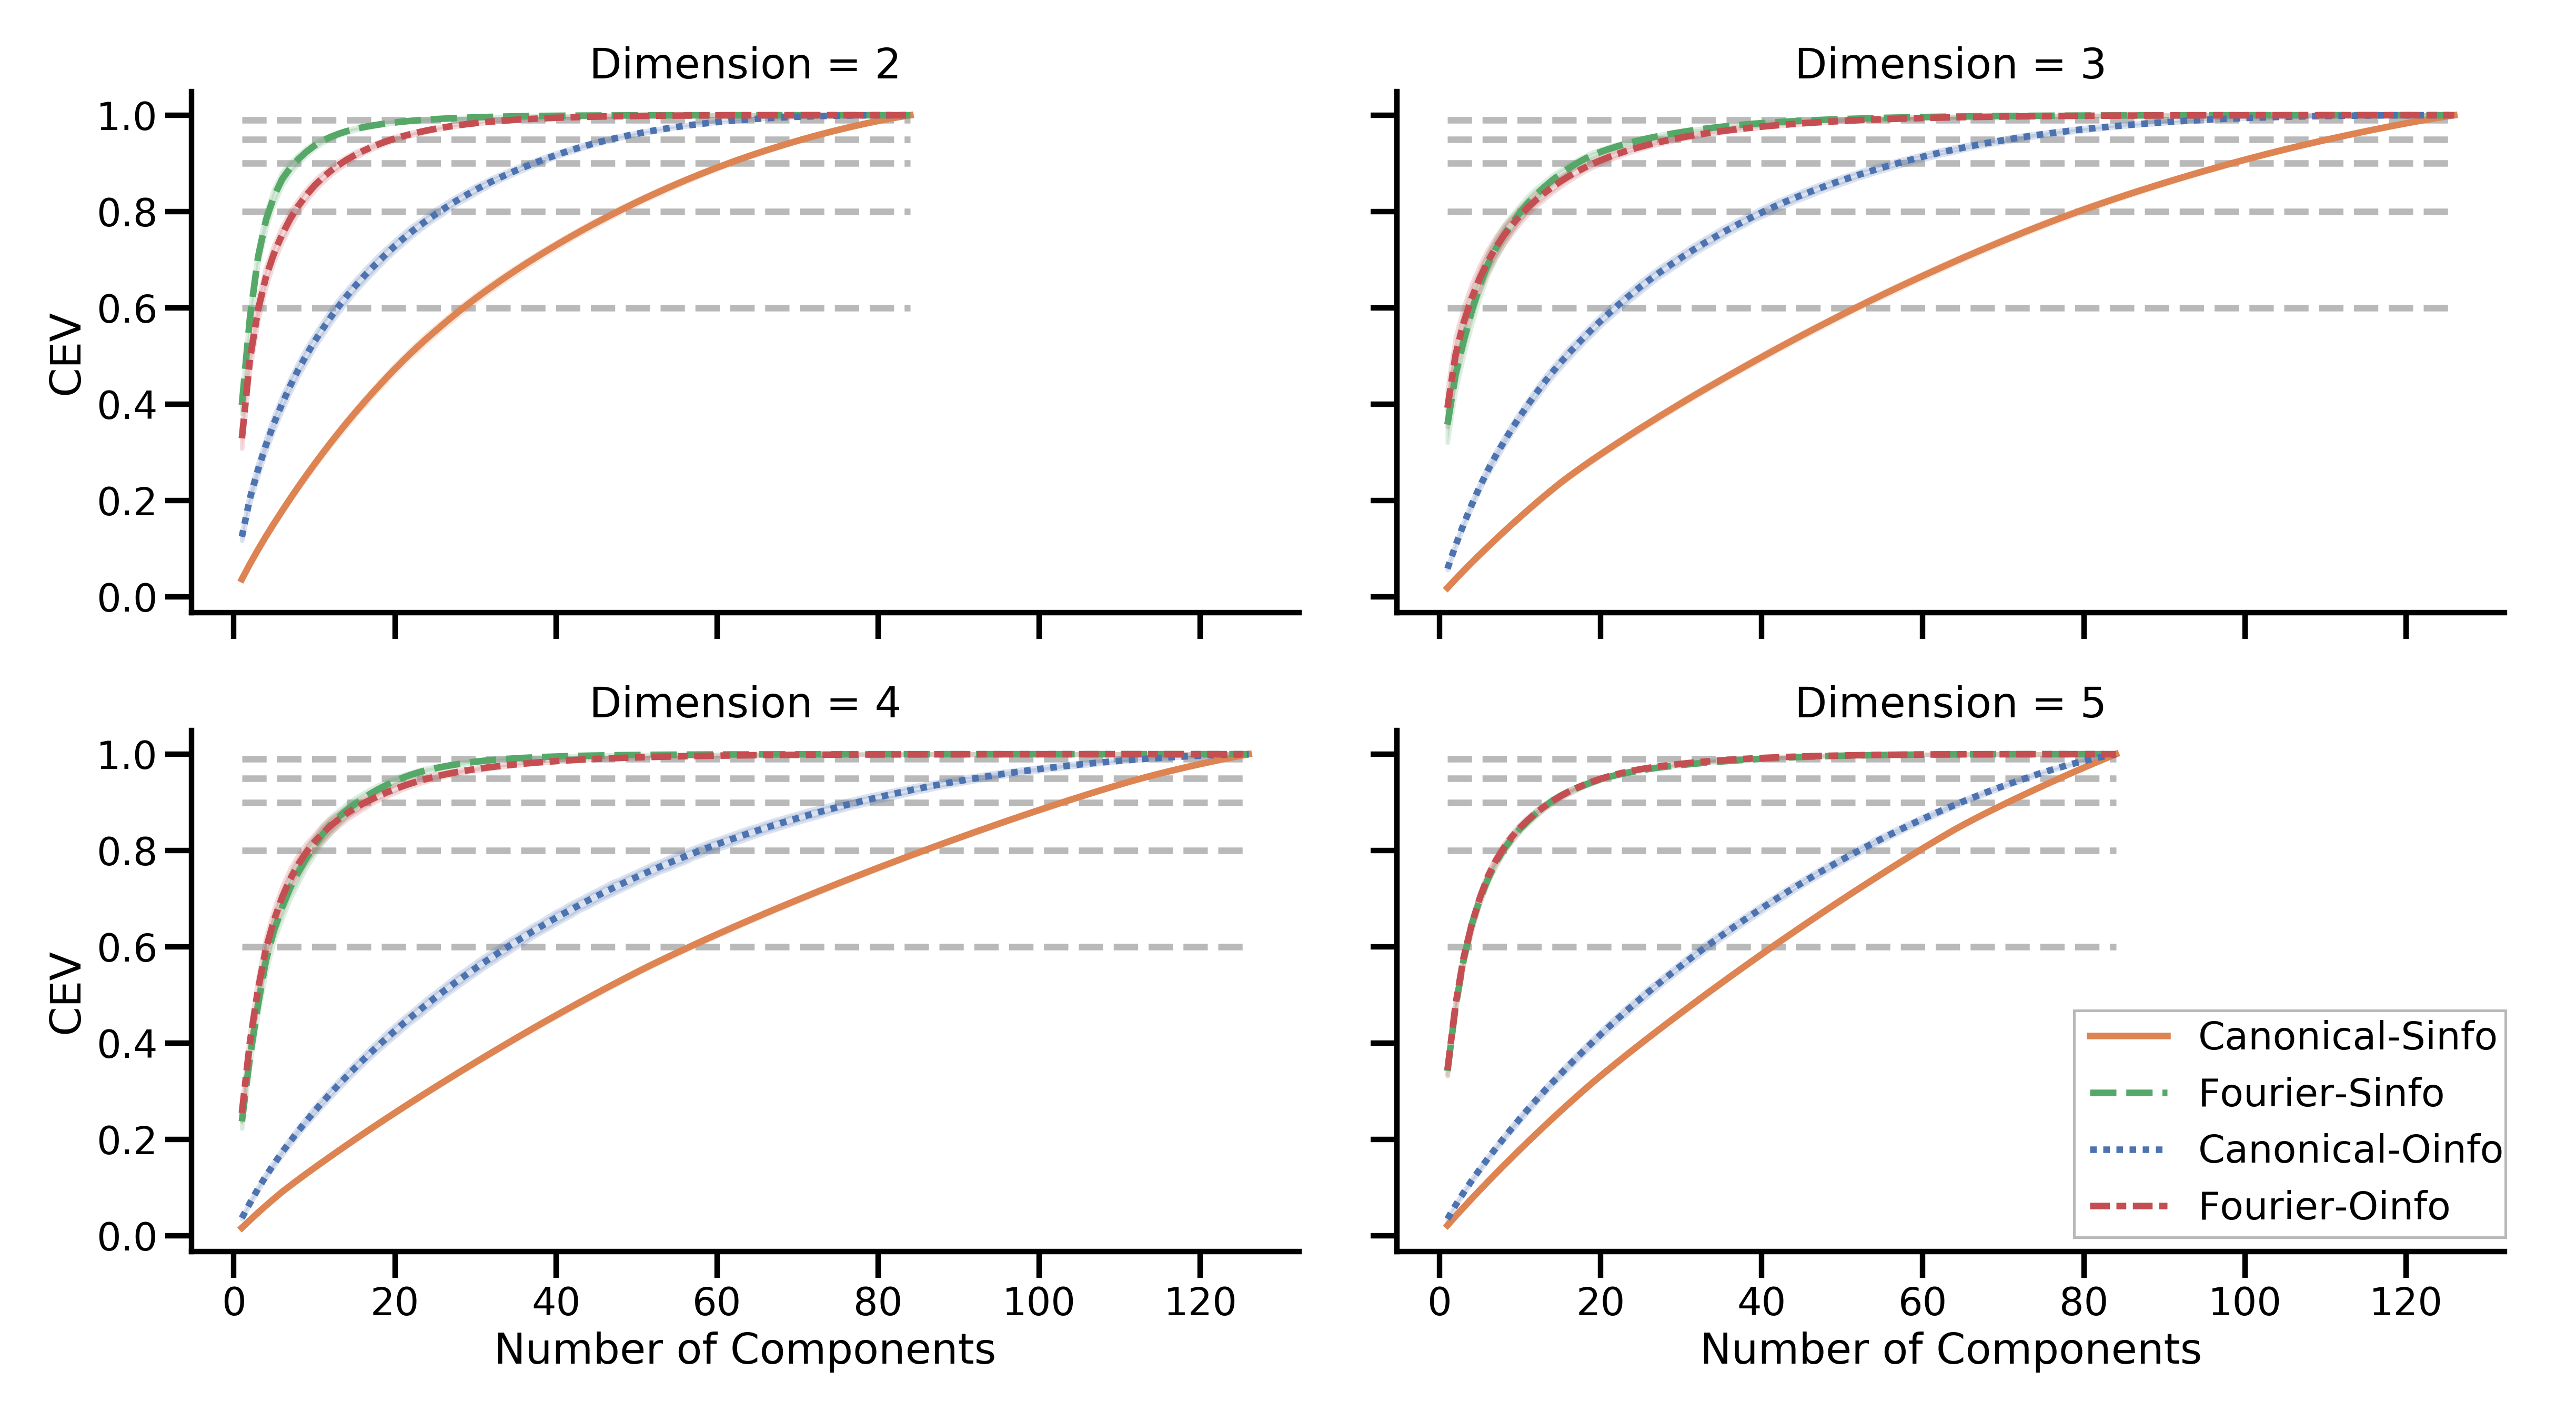
\includegraphics[scale=.096]{media/hyperharmonic}
\end{frame}